\section{ErrorMessageComponent Klassenreferenz}
\label{classErrorMessageComponent}\index{ErrorMessageComponent@{ErrorMessageComponent}}
Klassendiagramm für ErrorMessageComponent::\begin{figure}[H]
\begin{center}
\leavevmode
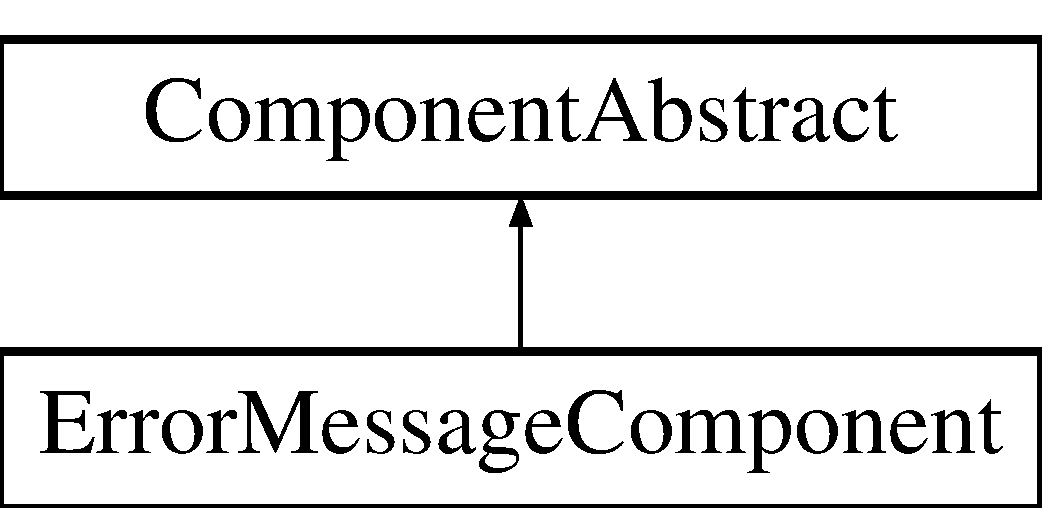
\includegraphics[height=2cm]{classErrorMessageComponent}
\end{center}
\end{figure}
\subsection*{Öffentliche Methoden}
\begin{CompactItemize}
\item 
{\bf ErrorMessageComponent} (\$instanceID, \$instanceName, \&\$smartyObj)
\item 
{\bf redender} ()
\item 
{\bf getOutput} ()
\end{CompactItemize}


\subsection{Ausführliche Beschreibung}


Definiert in Zeile 7 der Datei ErrorMessageComponent.php.

\subsection{Dokumentation der Elementfunktionen}
\index{ErrorMessageComponent@{ErrorMessageComponent}!ErrorMessageComponent@{ErrorMessageComponent}}
\index{ErrorMessageComponent@{ErrorMessageComponent}!ErrorMessageComponent@{ErrorMessageComponent}}
\subsubsection{\setlength{\rightskip}{0pt plus 5cm}ErrorMessageComponent.ErrorMessageComponent (\$ {\em instanceID}, \$ {\em instanceName}, \&\$ {\em smartyObj})}\label{classErrorMessageComponent_6a7ed825ae570b558d327b6755fd9def}




Definiert in Zeile 9 der Datei ErrorMessageComponent.php.\index{ErrorMessageComponent@{ErrorMessageComponent}!redender@{redender}}
\index{redender@{redender}!ErrorMessageComponent@{ErrorMessageComponent}}
\subsubsection{\setlength{\rightskip}{0pt plus 5cm}ErrorMessageComponent.redender ()}\label{classErrorMessageComponent_52fef8c30b1f7359629e35d179e0663b}


Redender component 

Definiert in Zeile 17 der Datei ErrorMessageComponent.php.\index{ErrorMessageComponent@{ErrorMessageComponent}!getOutput@{getOutput}}
\index{getOutput@{getOutput}!ErrorMessageComponent@{ErrorMessageComponent}}
\subsubsection{\setlength{\rightskip}{0pt plus 5cm}ErrorMessageComponent.getOutput ()}\label{classErrorMessageComponent_09fb53a235cb49ba3da7ff55c8f4b777}


return string of redendered component

\begin{Desc}
\item[Rückgabe:]string \end{Desc}


Definiert in Zeile 33 der Datei ErrorMessageComponent.php.

Die Dokumentation für diese Klasse wurde erzeugt aufgrund der Datei:\begin{CompactItemize}
\item 
{\bf ErrorMessageComponent.php}\end{CompactItemize}
